\documentclass{beamer}
\usepackage[utf8]{inputenc}
\usepackage{graphicx}
\usepackage{amsmath}
\usepackage{bibentry}


\AtBeginSection[]{
  \begin{frame}
  \vfill
  \centering
  \begin{beamercolorbox}[sep=8pt,center,shadow=true,rounded=true]{title}
    \usebeamerfont{title}\insertsectionhead\par%
  \end{beamercolorbox}
  \vfill
  \end{frame}
}

\title{Incentivos al Retiro}

\begin{document}

\begin{frame}
\maketitle
\end{frame}



\frame
{
  \frametitle{Primeros Resultados}
  \begin{itemize}
  \item Los primeros trabajos que miden los efectos de la Seguridad Social sobre el mercado de trabajo son de los años 80s.
  \item Hacia fines del siglo pasado, había considerable evidencia de que en los países de la OCDE, los incentivos generados por los sistemas de seguridad social eran un factor determinante en la baja de la participación laboral de los hombre mayores.
  \end{itemize}
}



\frame
{
  \frametitle{Primeros estudios}
  \begin{itemize}
  \item Se basan en estimaciones cross-section.
  \item Se calculan incentivos de retiro (\textit{SSW, Peak Value, etc.}) y se estiman modelos usando datos cross-section.
  \item Varios trabajos documentaron que los sistemas previsonales penalizaban fuertemente el trabajo luego de tener causal.
  \item Este impuesto implícito sobre la actividad laboral de los mayores tiene efectos sobre las tasas de actividad.
  \item No permitían identificar con precisión el impacto de distintos parámetros de los sistemas.
  \end{itemize}
}

\frame
{
  \frametitle{Evidencia OCDE}
  Microestimation, Alemania, algún otro?
}

\frame
{
  \frametitle{Evidencia América Latina}
  \begin{itemize}
  \item Chile (Cerdas 2005)
  \item Méjico (Aguila, Miranda-Muñoz)
  \item Brasil
  \end{itemize}
}

\frame
{
  \frametitle{Orientación general de las políticas}
  
  OCDE vs. América Latina
  
  
}



\frame
{
  \frametitle{Problemas}
  
  ~\cite{mastrobouni09} discute las limitaciones de esta literatura:
  \begin{itemize}
  \item Endogeneidad
  \item Error de medida
  \item No captura efectos de señalización de las edades de retiro.
  \end{itemize}
}

\frame
{
  \frametitle{Trabajos Recientes}
  
  \begin{itemize}
  \item La literatura más reciente busca evaluar los efectos de las políticas de los últimas décadas, que buscaron estimular la oferta de trabajo de los mayores.
  \item Usan registros administrativos y metodologías cuasi-expermientales para medir los impactos de los cambios paramétricos en:
    \begin{itemize}
     \item Las edades de retiro efectivas
     \item La oferta laboral
     \item El uso de otros programas de seguridad social
     \item La salud (escasa evidencia)
     \item La oferta laboral de los cónyuges
     \end{itemize}
  \end{itemize}
}

\frame
{
  \frametitle{Metodos cuasi-experimentales}
  
}
\frame
{
  \frametitle{Edad Mínima de Retiro (EMR)}

    \begin{itemize}
    \item Rabaté 2018 - Francia
    \item Staubli 2011 - Austria
    \item Atalay 2012 - Australia
    \item Cribb 2016 - UK
    \item Geyer 2018 - Alemania
    \item Vestad 2013 - Noruega
    \end{itemize}
}
  \frame
  {
    \frametitle{Edad normal de retiro (ENR)/Ajustes actuariales}
    \begin{itemize}
    \item Lalive 2015 - Suiza
    \item Hanel 2012 - Suiza
    \item Hanel 2009 - Alemania
    \item Mastrobouni 2009 - EUA
    \end{itemize}
  }

  \frame
  {
     \frametitle{Rabaté 2018}
     \begin{itemize}
       \item Employment and substitution effects of raising the statutory retirement age in France.
       \item Francia, \textit{Régime Général}, cubre $\frac{2}{3}$ de la población.
       \item Suba gradual de la EMR de 60 a 62 a partir 2010.
       \item Hay un cambio en la ENR que afecta otras cohortes (no se evalúa).
     \end{itemize}
  }
  \frame
  {
    \frametitle{Identificación}
      \begin{itemize}
        \item Evalúa el impacto de la suba de 60 a 61 sobre oferta laboral y sustitución por otros programas.
        \item La primera cohorte afectada es la nacida a finales de 1951, su EMR pasó a 60 años y 4 meses.
       \item La cohorte 1955 tiene una EMR de 62 años.
     \end{itemize}
  }
  \frame
  {
    \frametitle{Evidencia Descriptiva}
      \begin{figure}[htp]
        \centering
        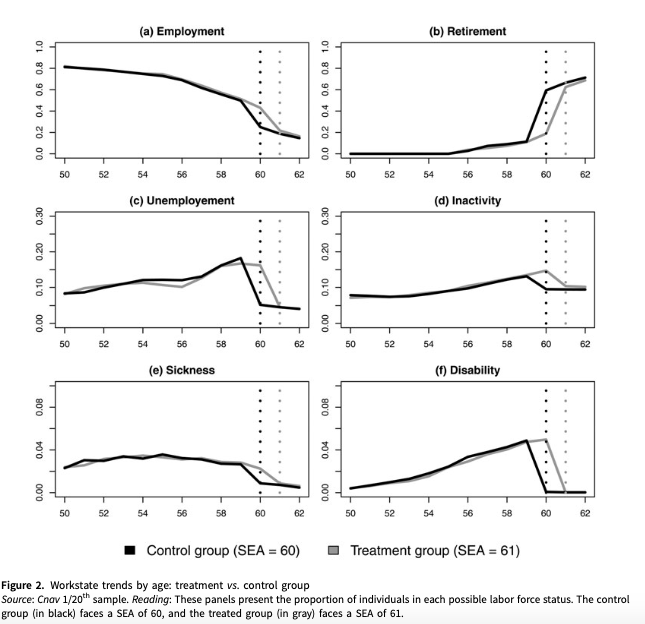
\includegraphics[width=8cm]{imgs/rabate-fig2}
        \label{fig:fig2}
      \end{figure}
  }
  \frame
  {
    \frametitle{Evidencia Descriptiva}
    La cohorte tratada ...
        \begin{itemize}
        \item  menor probabilidad de retirarse (los trabajadores menores de la EMR pueden retirarse si tienen carreras de trabajo largas).
        \item  mayor probabilidad de estar trabajando.
        \item  mayor probabilidad de estar desempleados.
        \item  mayor probabilidad de estar inactivos, en seguro de enfermedad e invalidez.
     \end{itemize}
    
  }
  \frame
  {
    \frametitle{Resultados}
      \begin{figure}[htp]
        \centering
        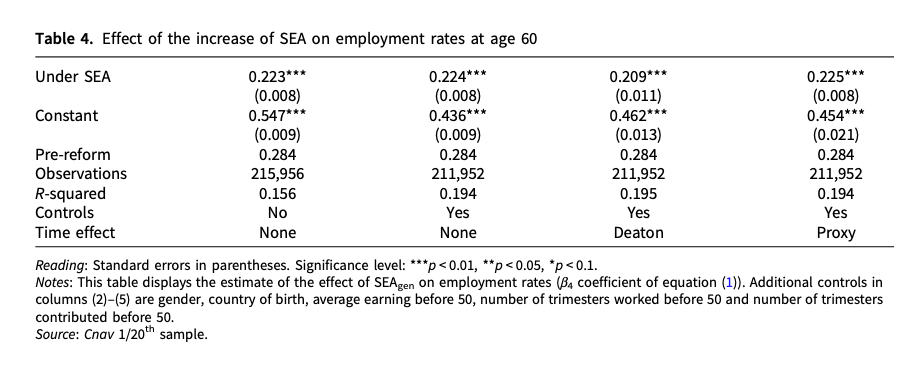
\includegraphics[width=12cm]{imgs/rabate-tab4}
        \label{fig:fig2}
      \end{figure}
  }
  \frame
  {
    \frametitle{Resultados(2)}
      \begin{figure}[htp]
        \centering
        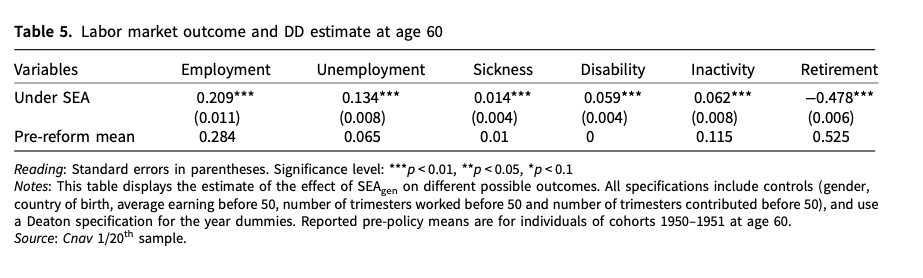
\includegraphics[width=12cm]{imgs/rabate-tab5}
        \label{fig:fig2}
      \end{figure}
  }
  \frame
  {
    \frametitle{Discusión}
      Permiten establecer efectos causales de aumentar la EMR.
      \begin{itemize}
      \item La probabilidad de estar empleado sube aprox. 20\%.
      \item El principal efecto sustitución es con el seguro de desempleo (13.5 \%)
      \item Efectos menores pero significativos sobre invalidez, enfermedad e inactividad.
      \end{itemize}
  }
  \frame
  {
    \frametitle{Efectos Heterogéneos}
        \begin{figure}[htp]
        \centering
        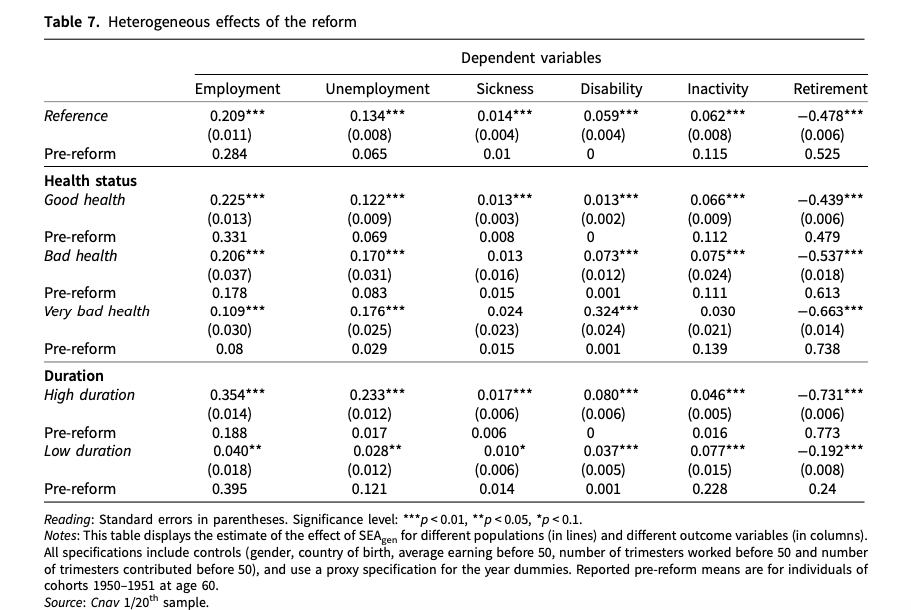
\includegraphics[width=12cm]{imgs/rabate-tab7}
        \label{fig:fig2}
      \end{figure}
  }
  \frame
  {
    \frametitle{Heterogeneidad}
  }
  
  \frame
  {
    \frametitle{Staubli y Zweimüller (2011 - IZA)}
    \begin{itemize}
    \item Does Raising the Retirement Age Increase Employment of Older Workers?
    \item Austria, aumento de la ERA en 2000 y 2004
    \item Estima los efectos sobre el empleo y el uso de otros programas de Seguridad Social.
    \end{itemize}
  }
  \frame
  {
    \frametitle{Contexto}
    \begin{itemize}
    \item En 2000, baja participación de mayores en el mercado laboral.
    \item EMR son 55 y 60 para hombres y mujeres respectivamente.
    \item El sistema público cubre a casi todos los trabajadores del país.
    \item Ofrece seguro de desempleo e invalidez.
    \end{itemize}
  }
  \frame
  {
    \frametitle{Reforma de 2000}
    \begin{itemize}
    \item La edad de retiro aumenta 1.5 años en forma gradual (Los hombres (mujeres) nacidos en Setiembre de 1940 (1945) aumentan 2 meses su EMR.
    \item Luego, cada trimestre sube 2 meses hasta llegar a 18 meses.
    \item Los hombres (mujeres) con más de 45 (40) años de trabajo no se ven afectados.
    \item La penalización por retirarse antes de la ENR también aumentó.
    \end{itemize}
  }
    \frame
  {
    \frametitle{Reforma de 2004}
    \begin{itemize}
    \item La edad de retiro vuelve a aumentar gradualmente a 65 y 60 años.
 
    \item Este cambio afecta a hombres nacidos a partir del primer semestre de  1943 para los hombres y 1948 las mujeres.
    \end{itemize}
  }
  \frame
  {
    \frametitle{Evidencia Descriptiva}
      \begin{figure}[htp]
        \centering
        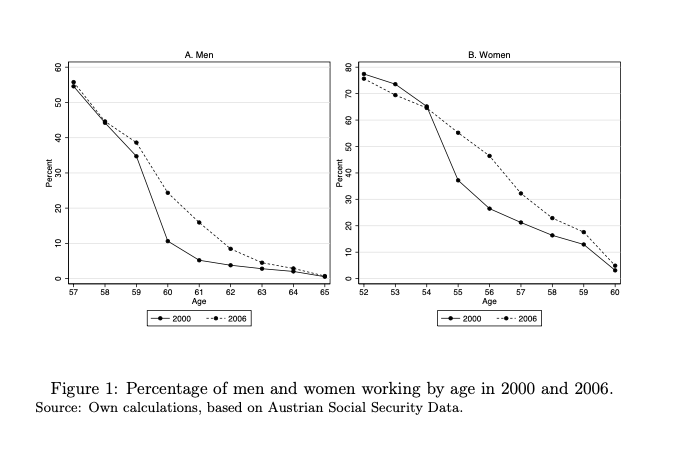
\includegraphics[width=10cm]{imgs/staubli-fig1}
        \label{fig:fig2}
        \caption{La proporción de hombres y mujeres trabajando aumenta entre 2000 y 2006 para todas las edades afectadas.}
      \end{figure}
  }
  \frame
  {
    \frametitle{Más evidencia descriptiva}
      \begin{figure}[htp]
        \centering
        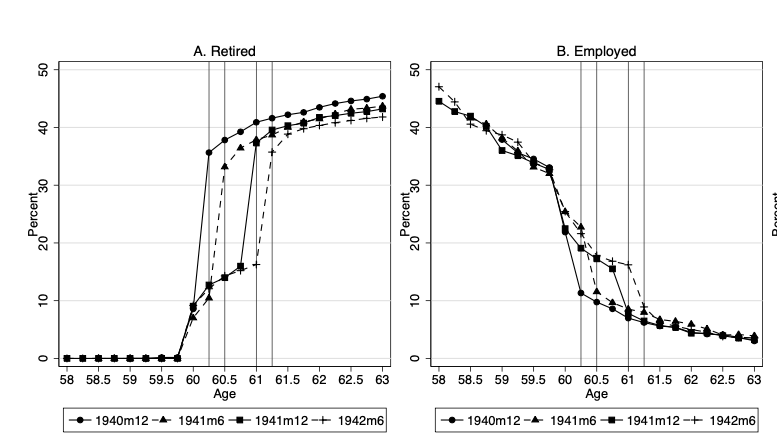
\includegraphics[width=10cm]{imgs/staubli-fig4}
        \caption{Saltos en las proporciones en la edad de cada cohorte}
        \label{fig:fig2}
      \end{figure}
  }
  \frame
  {
    \frametitle{Resultados}
      \begin{figure}[htp]
        \centering
        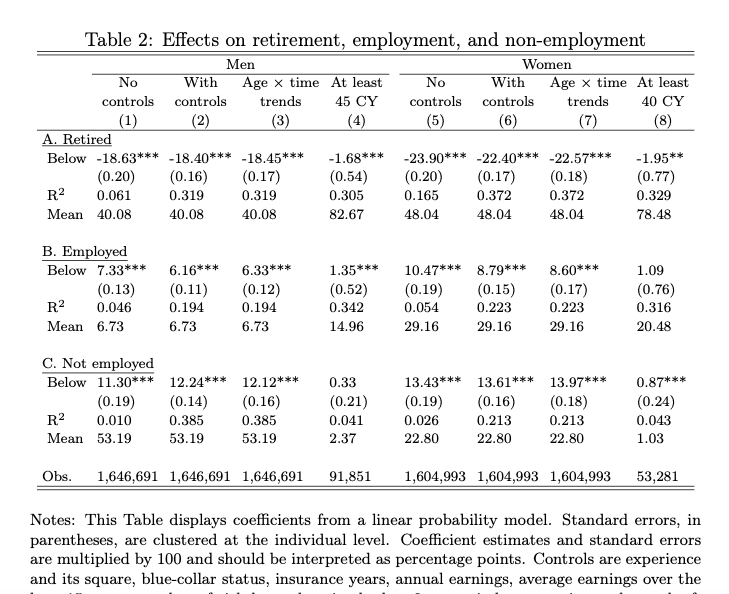
\includegraphics[width=10cm]{imgs/staubli-tab2}
        \caption{Salida 2}
        \label{fig:fig2}
      \end{figure}
  }
  \frame
  {
    \frametitle{Lectura}
    Estar bajo la EMR...
    \begin{itemize}
    \item ... baja la probabilidad de retirarse entre 18.5 \% (H) y 23 \% (M).
    \item ... sube la probabilidad de estar trabajando 7 \% (H) y 8-10 \% (M).
    \item ... sube la probabilidad de estar inactivo 11 \% (H) y 13 \% (M).         \end{itemize}
  }
  \frame
  {
    \frametitle{Salida 1}
      \begin{figure}[htp]
        \centering
        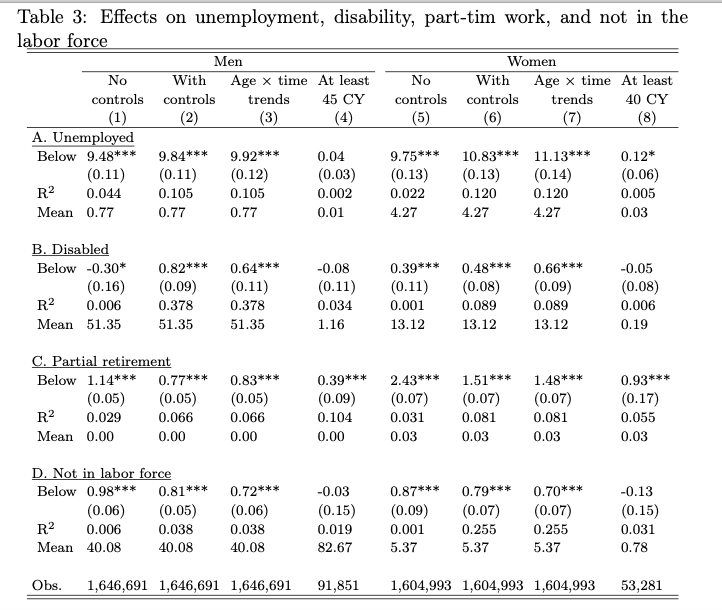
\includegraphics[width=10cm]{imgs/staubli-tab3}
        \caption{Salida 2}
        \label{fig:fig2}
      \end{figure}
  }
  \frame
  {
    \frametitle{Efectos sobre otros programas}
    \begin{itemize}
    \item Aumenta la probabilidad de estar desempleado.
    \item Aumenta la probabilidad de estar en retiro parcial.
    \item Aumenta la probabilidad de estar fuera del mercado.
    \item Aumenta la probabilidad de estar en en invalidez.
    \end{itemize}
  }
  \frame
    {
    \frametitle{Heterogeneidad: Salud y capital humano}
      \begin{figure}[htp]
        \centering
        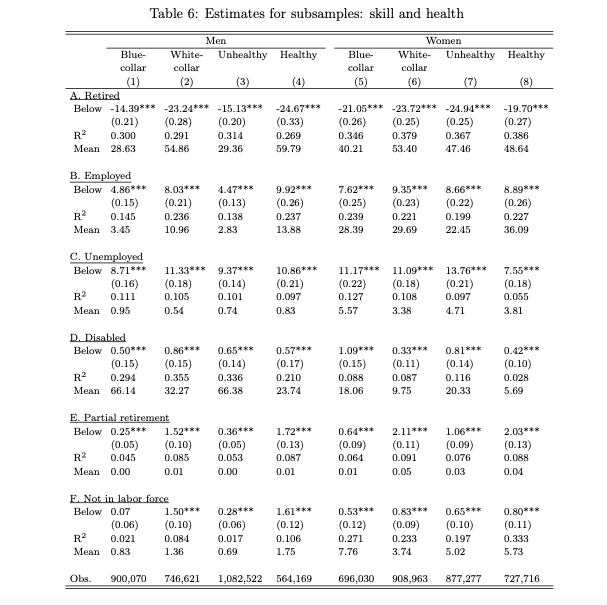
\includegraphics[width=10cm]{imgs/staubli-tab6}
        \caption{Salida 2}
        \label{fig:fig2}
      \end{figure}
  }
  \frame
    {
    \frametitle{Heterogeneidad: Ingresos}
      \begin{figure}[htp]
        \centering
        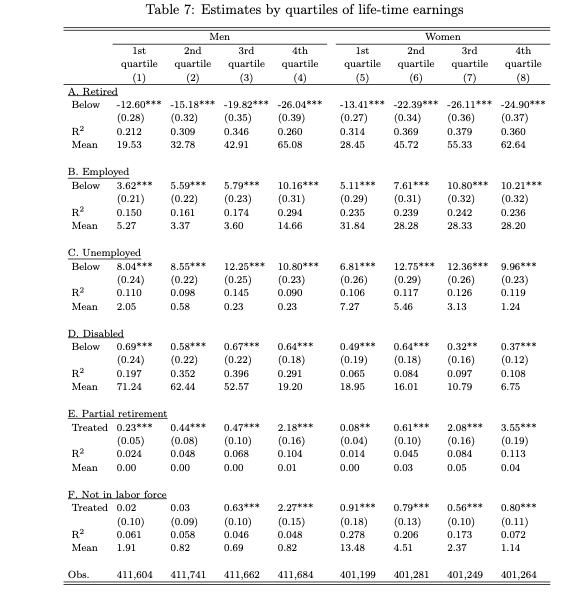
\includegraphics[width=10cm]{imgs/staubli-tab7}
        \caption{Salida 2}
        \label{fig:fig2}
      \end{figure}
  }
  

  \frame
   {
     \frametitle{Labour Supply effects of early retirement provision}
     \begin{itemize}
     \item Noruega
     \item Baja de la ERA de 64 a 62. 
     \end{itemize}
   }

       \frame
           {
             \frametitle{Política: AFP}
             \begin{itemize}
             \item Es un programa de retiro temprano voluntario al que acceden los trabajadores del sector público y la mitad de los trabajadores privados.
             \item Al principio la edad mínima era 66, se redujo gradualmente a 62 entre 1990 y 1998.
             \item La edad de retiro normal era 67, y antes de 1989 no había opciones de retiro temprano.
             \item Los programas de desempleo e invalidez funcionaban como vías de salida del mercado laboral.

             \end{itemize}
           }
      \frame
           {
             \frametitle{AFP: Beneficios}
             \begin{itemize}
             \item No hay ajustes actuariales
             \end{itemize}
           }
           
    \frame
    {
    \frametitle{Evidencia descriptiva}
    
    \begin{figure}[htp]
      \centering
      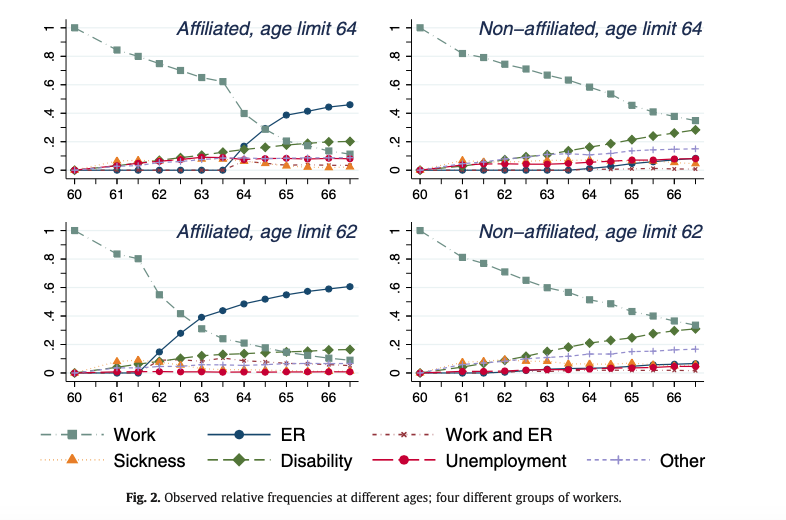
\includegraphics[width=8cm]{imgs/vestad-fig2}
      \caption{Descriptivos}
      \label{fig:fig2}
    \end{figure}
    }
           \frame {
             \frametitle{Estrategia empírica}
             \begin{itemize}
             \item Diff-in-diff usando el grupo de trabajadores con ERA 62 con el de ERA 64.
             \item $Y_{ict}$ es el estado relevante (trabajando, en seguro de desmpleo o en seguro de invalidez).
             \end{itemize}
             
             \begin{align*}
               y_{ict} &= \alpha + \beta_{1}X_{i} + \beta_{2} \tau_{t} + \beta_{3} \delta_{c} + \beta_{4}D_{i} \\
               &+ \beta_{5} (\delta_{c} \times \tau_{t}) + \beta_{6} ( D_{i} \times \tau_{t}) + \beta_{7} (D_{i} \times \tau_{t}) \\
               &+ \beta_{8} (\delta_{c} \times \tau_{t} \times D_{i})
             \end{align*}

           }

    \frame
    {
    \frametitle{Salida}
    
    \begin{figure}[htp]
      \centering
      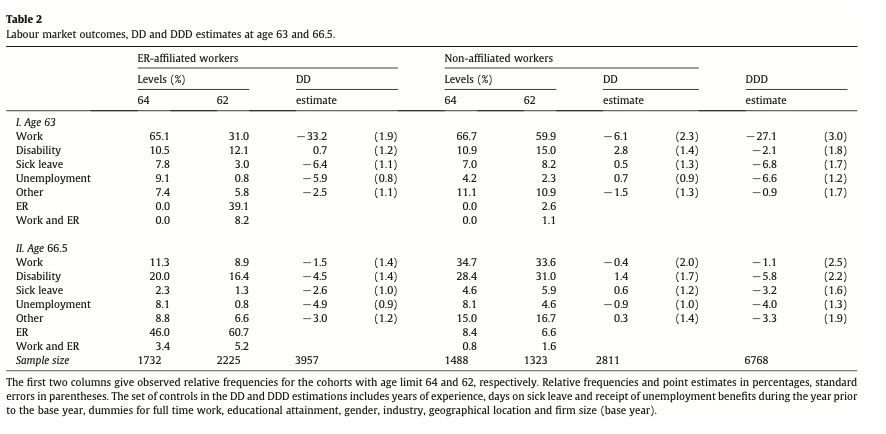
\includegraphics[width=14cm]{imgs/vestad-tbl2}
      \caption{Descriptivos}
      \label{fig:fig2}
    \end{figure}
    }
   \frame {
     \frametitle{Resultados y discusión}
        \begin{itemize}
        \item Se estiman los efectos en la oferta de trabajo de cambios en la edad mínima de retiro, caracterizando el impacto sobre distintos caminos hacia el retiro y la sustitución entre programas.
       \item La mitad de los jubilados por el programa de retiro temprano estarían trabajando a los 66.5 años sin el programa.
       \item 70\% estarían trabajando a los 63 si la edad fuera 64.
       \item El principal programa sustituto es la pensión por invalidez.
       \end{itemize}


}
              \frame
              {
                \frametitle{Atalay y Barrett, 2012}
                  \begin{itemize}
                  \item The Impact of Age Pension Eligibility Age on Retirement and Program Dependence: Evidence from an Australian Experiment
                  \item Australia, aumento gradual de la EMR de las mujeres en 1993.
                  \item Estima el impacto del cambio en la edad mínima de retiro en la oferta laboral.
                  \item Analiza la sustitución por otros programas de Seguridad Social.
                  \end{itemize}
              }
              \frame
              {
                \frametitle{Contexto}
                  \begin{itemize}
                  \item Se evalúan cambios al pilar no contributivo.
                  \item Este pilar tiene un test de ingresos y de \textit{assets}
                  \item Cubre al 69\% de la población.
                  \item EMR de 65 y 60 años para hombres y mujeres respectivamente.
                  \end{itemize}
               } 

              \frame
              {
                \frametitle{Reforma}
                
                \begin{itemize}
                \item Transición hacia igualar las EMR  para 2014.
                \item A partir de Julio de 1995, la EMR de las mujeres aumenta 6 meses cada 2 años.
                \item Las mujeres que tienen una EMR de 65 años (nacidas a paritr de 1949) tienen una caída de la \textit{SSW} de 23\% respecto a las que enfrentan una EMR de 60 (nacidas en 1935 y antes. 
                \end{itemize}
              }
              \frame
              {
                \frametitle{Estrategia}
                Compara las tasas de retiro de las cohortes afectadas con las de las cohortes no afectadas y los hombres.
              }
              \frame
              {
                  \begin{figure}[htp]
                  \centering
                  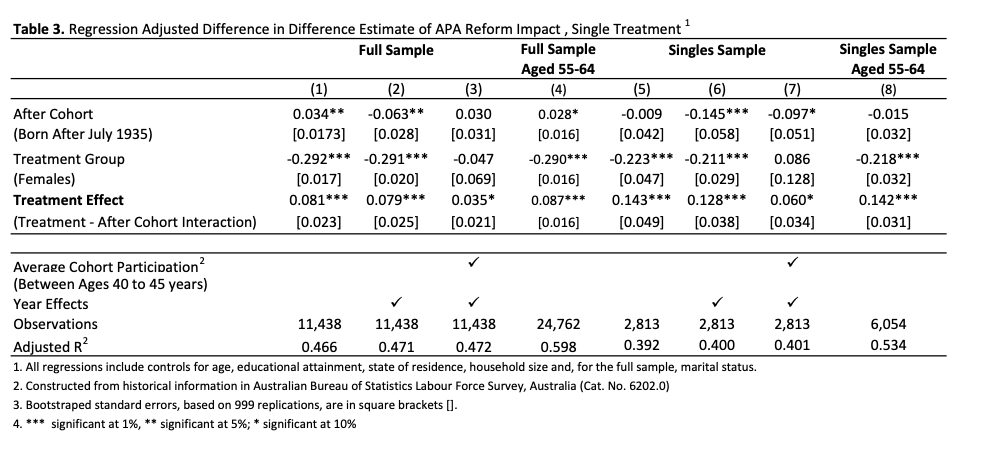
\includegraphics[width=10cm]{imgs/atalay-tab3}
                  \label{fig:fig2}
                  \end{figure}
    
              }
              \frame
              {
                \frametitle{Resultados}
                \begin{itemize}
                \item La participación laboral de las mujeres afectadas aumentó  8 \% .
                \item La probabilidad de cobrar una pensión por invalidez aumenta 12 \%.
                \end{itemize}
              }
              \frame
              {
              
              \frametitle{Cribb 2016 - UK}
              }
              \frame
              {
              
                \frametitle{Contexto}
              }
              \frame
              {
              
                \frametitle{Política}
              }
              \frame
              {
              
                \frametitle{Evidencia Descriptiva}
              }
                            \frame
              {
              
                \frametitle{Resultados}
              }
              \frame
              {
                \frametitle{Discusión}
              }
              
              \frame
              {
                \frametitle{Mastrobouni 2009 - EUA}
                  \begin{itemize}
                  \item Labor supply effects of the recent social security benefit cuts: Empirical estimates using cohort discontinuities.
                  \item Aumento de la NRA en EUA
                  \item Se aprueba en 1983, y empieza a regir a partir de 2000.
                  \item Las prestaciones se ajustan actuarialmente, cada dos meses de incremento en la ENR implica una reducción de aproximadamente 1\%.
                  \item Analiza el impacto sobre la edad de retiro efectiva.
                  \end{itemize}
}

 
  \frame
  {
    \frametitle{Evidencia Descriptiva}
      \begin{figure}[htp]
        \centering
        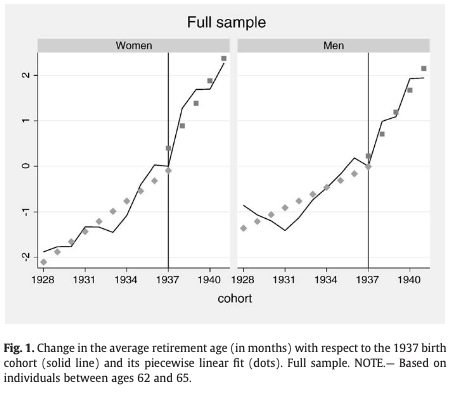
\includegraphics[width=8cm]{imgs/mastrobouni-fig1}
        \caption{El aumento en la edad efectiva de retiro se acelera para las cohortes afectadas}
        \label{fig:fig2}
      \end{figure}
  }
  \frame
  {
    \frametitle{Estrategia}
    \begin{itemize}
      \item Diff-in-diff
      \item Cohortes 1928-1937 (control)
      \item Cohortes 1938-1941 (tratamiento)
      \item 3 formas de corregir errores de clasificación por la fecha de nacimiento (\textit{naive, sophisticated y restricted})
    \end{itemize}
  }
  \frame
  {
    \frametitle{Resultados}
      \begin{figure}[htp]
        \centering
        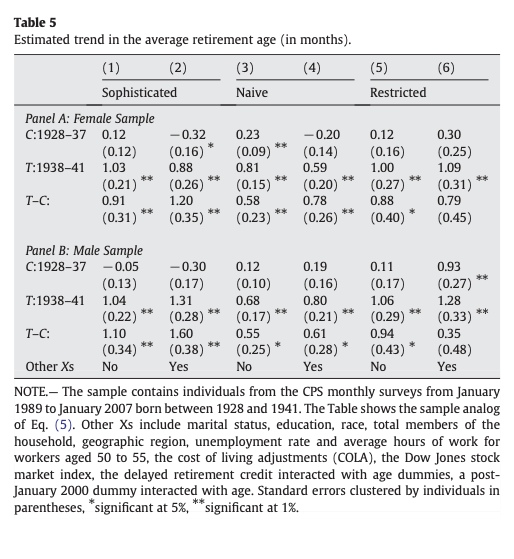
\includegraphics[width=8cm]{imgs/mastrobouni-tab5}
        \label{fig:fig2}
      \end{figure}
  }
  \frame
  {
    \frametitle{Discusión}
    \begin{itemize}
      \item El crecimiento de la edad promedio de retiro se acelera para los cohortes que enfrentan la nueva NRA.
      \item La diferencia estimada en la pendiente es (1.10 y 0.94) por año.
      \item Como cada año la NRA aumenta 2 meses, la edad efectiva de retiro aumenta 50\% del aumento de la NRA.
    \end{itemize}
  }
  \frame
  {
    \frametitle{Heterogeneidad}
    
    \begin{itemize}
    
    \item Los hombres con solo secundaria terminada son el subgrupo que reacciona más a los incentivos.
    \end{itemize}
  }
  \frame
  {
    \frametitle{Hanel 2010}
    \begin{itemize}
    \item Financial incentives to postpone retirement and further effects on employment
    \item Alemania, sistema de reparto que cubre 33.5 millones de trabajadores privados.
    \item Desde 1972 existen varias formas de retirarse a partir de los 60 sin penalizaciones (pensión para mujeres, desempleados, inválidos).
    \end{itemize}
  }
  \frame
  {
    \frametitle{Cambios 1997}
    \begin{itemize}
      \item Se implementen deducciones en las prestaciones de 0.3\% por mes antes de la ENR en que se solicita la jubilación.
      \item Se implementa gradualmente por cohortes (los hombres nacidos en Enero de 1938 tienen una ENR de 60 y 1 mes).
    \end{itemize}
  }
  \frame
  {
    \frametitle{Evidencia Descriptiva}
      \begin{figure}[htp]
        \centering
        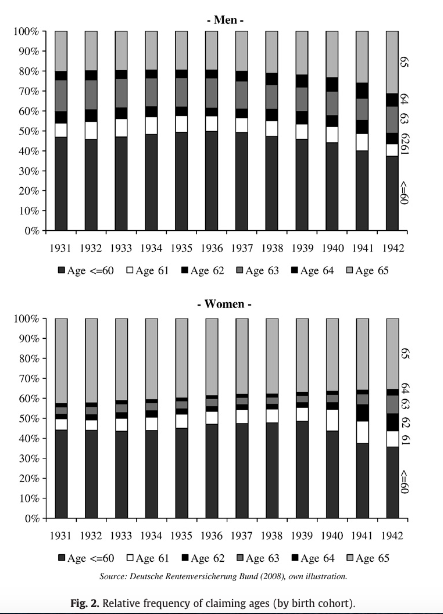
\includegraphics[width=6cm]{imgs/hanel10-fig2}
        \label{fig:fig2}
      \end{figure}
  }
  \frame
  {
    \frametitle{Evidencia Descriptiva}
      
      \begin{itemize}
        \item La proporción de hombres que se jubila a los 65 es estable hasta la última cohorte no afectada (1937).
        \item En las cohortes afectadas la proporción aumenta.
        \item Para las mujeres, la primera cohorte afectada es la nacida en 1940.
        \item La proporción de mujeres retiradas a los 60 se reduce a partir de la introducción de los cambios.
      \end{itemize}
  }
  \frame
  {
    \frametitle{Análisis de supervivencia}
    \begin{itemize}
    \item Estima el impacto de la reforma en la probabilidad de dejar de trabajar y de pedir una jubilación en función de indicadores de incentivos.
    \item Para interpretar los resutados, reporta el cambio en el tiempo esperado para que sucedan esos eventos, controlando por las variables demográficas.
    \end{itemize}
  }
  % \frame
  % {
  %   \frametitle{Resultados}
  %     \begin{figure}[htp]
  %       \centering
  %       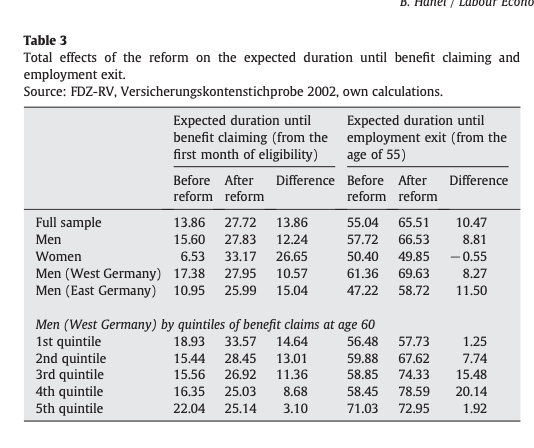
\includegraphics[width=10cm]{imgs/hanel10-tab3}
  %       \caption{Salida 2}
  %       \label{fig:fig2}
  %     \end{figure}
  % }
  \frame
  {
  \frametitle{Duración}
     \begin{itemize}
       \item La reforma aumenta 14 meses el tiempo que transcurre entre que el trabajador es elegible y solicita la jubilación.
       \item La reforma aumenta 10 meses el tiempo en que el trabajador permanece empleado después de los 55 años en 10.5 meses.
     \end{itemize}
  }
  \frame
  {
  \frametitle{Comentarios}
    \begin{itemize}
      \item Las mujeres reaccionan más que los hombres en la decisión de jubilación y menos en la decisión de dejar el trabajo.
      \item Los impactos sobre pedir una pensión son mayores que sobre dejar el empleo.
      \item Cuanto mayores los ingresos, menor es el impacto de la reforma en el tiempo hasta jubilarse, y mayor en el tiempo hasta dejar el trabajo.
    \end{itemize}

}

\frame
{
  \frametitle{Hanel 2012}
  \begin{itemize}
  \item Suiza
  \end{itemize}
}

\frame
{
  \frametitle{Contexto}
}

\frame
{
  \frametitle{Política}
}
\frame
{
  \frametitle{Resultados}
}
\frame
{
  \frametitle{Discusión}
}
              
\begin{frame}
\frametitle{References}
\footnotesize{
\begin{thebibliography}{99} % Beamer does not support BibTeX so references must be nserted manually as below
\bibitem[Mastrobouni, 2009]{p1} Giovanni Mastrobouni (2009)
\newblock Labor supply effects of the recent social security benefit cuts: empirical estimates using cohort discontinuities.
\newblock \emph{Journal Name} 12(3), 45 -- 678.
\end{thebibliography}
}
\end{frame}

\begin{frame}[t, allowframebreaks]
\frametitle{References}
\bibliographystyle{amsalpha}
\bibliography{referencias}
\end{frame}


\end{document}
